\documentclass[1p]{elsarticle_modified}
%\bibliographystyle{elsarticle-num}

%\usepackage[colorlinks]{hyperref}
%\usepackage{abbrmath_seonhwa} %\Abb, \Ascr, \Acal ,\Abf, \Afrak
\usepackage{amsfonts}
\usepackage{amssymb}
\usepackage{amsmath}
\usepackage{amsthm}
\usepackage{scalefnt}
\usepackage{amsbsy}
\usepackage{kotex}
\usepackage{caption}
\usepackage{subfig}
\usepackage{color}
\usepackage{graphicx}
\usepackage{xcolor} %% white, black, red, green, blue, cyan, magenta, yellow
\usepackage{float}
\usepackage{setspace}
\usepackage{hyperref}

\usepackage{tikz}
\usetikzlibrary{arrows}

\usepackage{multirow}
\usepackage{array} % fixed length table
\usepackage{hhline}

%%%%%%%%%%%%%%%%%%%%%
\makeatletter
\renewcommand*\env@matrix[1][\arraystretch]{%
	\edef\arraystretch{#1}%
	\hskip -\arraycolsep
	\let\@ifnextchar\new@ifnextchar
	\array{*\c@MaxMatrixCols c}}
\makeatother %https://tex.stackexchange.com/questions/14071/how-can-i-increase-the-line-spacing-in-a-matrix
%%%%%%%%%%%%%%%

\usepackage[normalem]{ulem}

\newcommand{\msout}[1]{\ifmmode\text{\sout{\ensuremath{#1}}}\else\sout{#1}\fi}
%SOURCE: \msout is \stkout macro in https://tex.stackexchange.com/questions/20609/strikeout-in-math-mode

\newcommand{\cancel}[1]{
	\ifmmode
	{\color{red}\msout{#1}}
	\else
	{\color{red}\sout{#1}}
	\fi
}

\newcommand{\add}[1]{
	{\color{blue}\uwave{#1}}
}

\newcommand{\replace}[2]{
	\ifmmode
	{\color{red}\msout{#1}}{\color{blue}\uwave{#2}}
	\else
	{\color{red}\sout{#1}}{\color{blue}\uwave{#2}}
	\fi
}

\newcommand{\Sol}{\mathcal{S}} %segment
\newcommand{\D}{D} %diagram
\newcommand{\A}{\mathcal{A}} %arc


%%%%%%%%%%%%%%%%%%%%%%%%%%%%%5 test

\def\sl{\operatorname{\textup{SL}}(2,\Cbb)}
\def\psl{\operatorname{\textup{PSL}}(2,\Cbb)}
\def\quan{\mkern 1mu \triangleright \mkern 1mu}

\theoremstyle{definition}
\newtheorem{thm}{Theorem}[section]
\newtheorem{prop}[thm]{Proposition}
\newtheorem{lem}[thm]{Lemma}
\newtheorem{ques}[thm]{Question}
\newtheorem{cor}[thm]{Corollary}
\newtheorem{defn}[thm]{Definition}
\newtheorem{exam}[thm]{Example}
\newtheorem{rmk}[thm]{Remark}
\newtheorem{alg}[thm]{Algorithm}

\newcommand{\I}{\sqrt{-1}}
\begin{document}

%\begin{frontmatter}
%
%\title{Boundary parabolic representations of knots up to 8 crossings}
%
%%% Group authors per affiliation:
%\author{Yunhi Cho} 
%\address{Department of Mathematics, University of Seoul, Seoul, Korea}
%\ead{yhcho@uos.ac.kr}
%
%
%\author{Seonhwa Kim} %\fnref{s_kim}}
%\address{Center for Geometry and Physics, Institute for Basic Science, Pohang, 37673, Korea}
%\ead{ryeona17@ibs.re.kr}
%
%\author{Hyuk Kim}
%\address{Department of Mathematical Sciences, Seoul National University, Seoul 08826, Korea}
%\ead{hyukkim@snu.ac.kr}
%
%\author{Seokbeom Yoon}
%\address{Department of Mathematical Sciences, Seoul National University, Seoul, 08826,  Korea}
%\ead{sbyoon15@snu.ac.kr}
%
%\begin{abstract}
%We find all boundary parabolic representation of knots up to 8 crossings.
%
%\end{abstract}
%\begin{keyword}
%    \MSC[2010] 57M25 
%\end{keyword}
%
%\end{frontmatter}

%\linenumbers
%\tableofcontents
%
\newcommand\colored[1]{\textcolor{white}{\rule[-0.35ex]{0.8em}{1.4ex}}\kern-0.8em\color{red} #1}%
%\newcommand\colored[1]{\textcolor{white}{ #1}\kern-2.17ex	\textcolor{white}{ #1}\kern-1.81ex	\textcolor{white}{ #1}\kern-2.15ex\color{red}#1	}

{\Large $\underline{11n_{176}~(K11n_{176})}$}

\setlength{\tabcolsep}{10pt}
\renewcommand{\arraystretch}{1.6}
\vspace{1cm}\begin{tabular}{m{100pt}>{\centering\arraybackslash}m{274pt}}
\multirow{5}{120pt}{
	\centering
	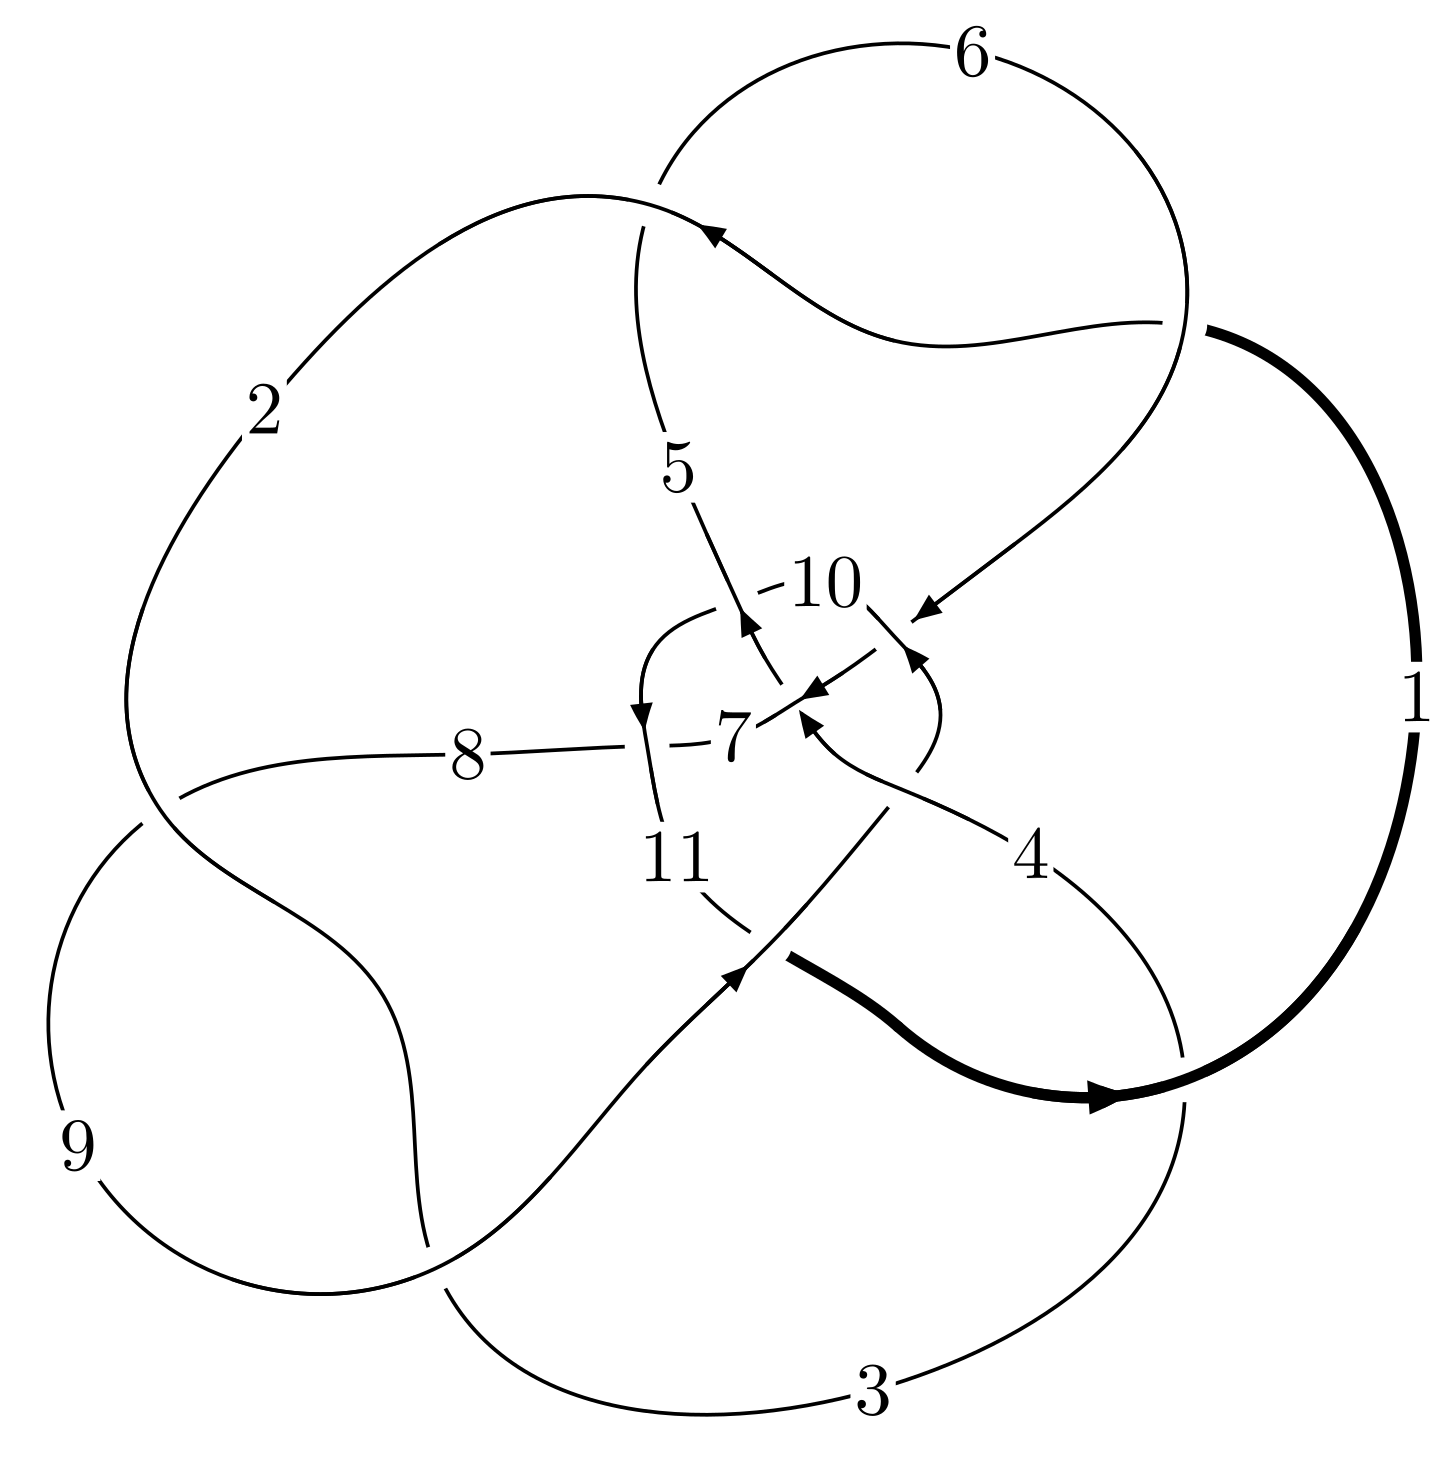
\includegraphics[width=112pt]{../../../GIT/diagram.site/Diagrams/png/792_11n_176.png}\\
\ \ \ A knot diagram\footnotemark}&
\allowdisplaybreaks
\textbf{Linearized knot diagam} \\
\cline{2-2}
 &
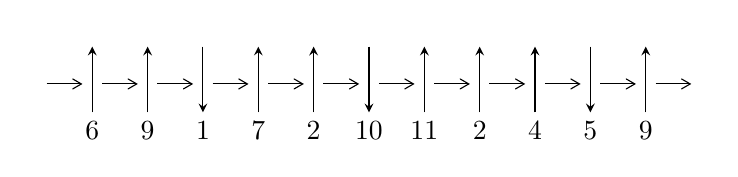
\begin{tikzpicture}[x=20pt, y=17pt]
	% nodes
	\node (C0) at (0, 0) {};
	\node (C1) at (1, 0) {};
	\node (C1U) at (1, +1) {};
	\node (C1D) at (1, -1) {6};

	\node (C2) at (2, 0) {};
	\node (C2U) at (2, +1) {};
	\node (C2D) at (2, -1) {9};

	\node (C3) at (3, 0) {};
	\node (C3U) at (3, +1) {};
	\node (C3D) at (3, -1) {1};

	\node (C4) at (4, 0) {};
	\node (C4U) at (4, +1) {};
	\node (C4D) at (4, -1) {7};

	\node (C5) at (5, 0) {};
	\node (C5U) at (5, +1) {};
	\node (C5D) at (5, -1) {2};

	\node (C6) at (6, 0) {};
	\node (C6U) at (6, +1) {};
	\node (C6D) at (6, -1) {10};

	\node (C7) at (7, 0) {};
	\node (C7U) at (7, +1) {};
	\node (C7D) at (7, -1) {11};

	\node (C8) at (8, 0) {};
	\node (C8U) at (8, +1) {};
	\node (C8D) at (8, -1) {2};

	\node (C9) at (9, 0) {};
	\node (C9U) at (9, +1) {};
	\node (C9D) at (9, -1) {4};

	\node (C10) at (10, 0) {};
	\node (C10U) at (10, +1) {};
	\node (C10D) at (10, -1) {5};

	\node (C11) at (11, 0) {};
	\node (C11U) at (11, +1) {};
	\node (C11D) at (11, -1) {9};
	\node (C12) at (12, 0) {};

	% arrows
	\draw[->,>={angle 60}]
	(C0) edge (C1) (C1) edge (C2) (C2) edge (C3) (C3) edge (C4) (C4) edge (C5) (C5) edge (C6) (C6) edge (C7) (C7) edge (C8) (C8) edge (C9) (C9) edge (C10) (C10) edge (C11) (C11) edge (C12) ;	\draw[->,>=stealth]
	(C1D) edge (C1U) (C2D) edge (C2U) (C3U) edge (C3D) (C4D) edge (C4U) (C5D) edge (C5U) (C6U) edge (C6D) (C7D) edge (C7U) (C8D) edge (C8U) (C9D) edge (C9U) (C10U) edge (C10D) (C11D) edge (C11U) ;
	\end{tikzpicture} \\
\hhline{~~} \\& 
\textbf{Solving Sequence} \\ \cline{2-2} 
 &
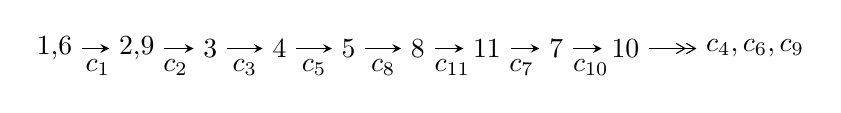
\begin{tikzpicture}[x=25pt, y=7pt]
	% node
	\node (A0) at (-1/8, 0) {1,6};
	\node (A1) at (17/16, 0) {2,9};
	\node (A2) at (17/8, 0) {3};
	\node (A3) at (25/8, 0) {4};
	\node (A4) at (33/8, 0) {5};
	\node (A5) at (41/8, 0) {8};
	\node (A6) at (49/8, 0) {11};
	\node (A7) at (57/8, 0) {7};
	\node (A8) at (65/8, 0) {10};
	\node (C1) at (1/2, -1) {$c_{1}$};
	\node (C2) at (13/8, -1) {$c_{2}$};
	\node (C3) at (21/8, -1) {$c_{3}$};
	\node (C4) at (29/8, -1) {$c_{5}$};
	\node (C5) at (37/8, -1) {$c_{8}$};
	\node (C6) at (45/8, -1) {$c_{11}$};
	\node (C7) at (53/8, -1) {$c_{7}$};
	\node (C8) at (61/8, -1) {$c_{10}$};
	\node (A9) at (10, 0) {$c_{4},c_{6},c_{9}$};

	% edge
	\draw[->,>=stealth]	
	(A0) edge (A1) (A1) edge (A2) (A2) edge (A3) (A3) edge (A4) (A4) edge (A5) (A5) edge (A6) (A6) edge (A7) (A7) edge (A8) ;
	\draw[->>,>={angle 60}]	
	(A8) edge (A9);
\end{tikzpicture} \\ 

\end{tabular} \\

\footnotetext{
The image of knot diagram is generated by the software ``\textbf{Draw programme}" developed by Andrew Bartholomew(\url{http://www.layer8.co.uk/maths/draw/index.htm\#Running-draw}), where we modified some parts for our purpose(\url{https://github.com/CATsTAILs/LinksPainter}).
}\phantom \\ \newline 
\centering \textbf{Ideals for irreducible components\footnotemark of $X_{\text{par}}$} 
 
\begin{align*}
I^u_{1}&=\langle 
9.28358\times10^{73} u^{46}+4.54756\times10^{74} u^{45}+\cdots+1.24850\times10^{77} b+1.15944\times10^{77},\\
\phantom{I^u_{1}}&\phantom{= \langle  }2.16945\times10^{75} u^{46}-2.78753\times10^{76} u^{45}+\cdots+3.74550\times10^{77} a-4.53039\times10^{78},\;u^{47}- u^{46}+\cdots-21 u+6\rangle \\
I^u_{2}&=\langle 
411 u^{15}+80 u^{14}+\cdots+327 b-544,\;1184 u^{15}+48 u^{14}+\cdots+327 a+175,\\
\phantom{I^u_{2}}&\phantom{= \langle  }u^{16}+4 u^{14}+u^{13}+3 u^{12}-10 u^{10}-9 u^9-30 u^8-19 u^7-33 u^6-18 u^5-21 u^4-10 u^3-7 u^2-2 u-1\rangle \\
\\
\end{align*}
\raggedright * 2 irreducible components of $\dim_{\mathbb{C}}=0$, with total 63 representations.\\
\footnotetext{All coefficients of polynomials are rational numbers. But the coefficients are sometimes approximated in decimal forms when there is not enough margin.}
\newpage
\renewcommand{\arraystretch}{1}
\centering \section*{I. $I^u_{1}= \langle 9.28\times10^{73} u^{46}+4.55\times10^{74} u^{45}+\cdots+1.25\times10^{77} b+1.16\times10^{77},\;2.17\times10^{75} u^{46}-2.79\times10^{76} u^{45}+\cdots+3.75\times10^{77} a-4.53\times10^{78},\;u^{47}- u^{46}+\cdots-21 u+6 \rangle$}
\flushleft \textbf{(i) Arc colorings}\\
\begin{tabular}{m{7pt} m{180pt} m{7pt} m{180pt} }
\flushright $a_{1}=$&$\begin{pmatrix}1\\0\end{pmatrix}$ \\
\flushright $a_{6}=$&$\begin{pmatrix}0\\u\end{pmatrix}$ \\
\flushright $a_{2}=$&$\begin{pmatrix}1\\- u^2\end{pmatrix}$ \\
\flushright $a_{9}=$&$\begin{pmatrix}-0.00579214 u^{46}+0.0744235 u^{45}+\cdots+7.90890 u+12.0956\\-0.000743579 u^{46}-0.00364242 u^{45}+\cdots+0.922897 u-0.928667\end{pmatrix}$ \\
\flushright $a_{3}=$&$\begin{pmatrix}-0.0143049 u^{46}+0.0978976 u^{45}+\cdots+4.71215 u+13.6102\\0.0228505 u^{46}-0.0369206 u^{45}+\cdots+1.75270 u-0.870753\end{pmatrix}$ \\
\flushright $a_{4}=$&$\begin{pmatrix}-0.0371555 u^{46}+0.134818 u^{45}+\cdots+2.95945 u+14.4810\\0.0228505 u^{46}-0.0369206 u^{45}+\cdots+1.75270 u-0.870753\end{pmatrix}$ \\
\flushright $a_{5}=$&$\begin{pmatrix}- u\\u^3+u\end{pmatrix}$ \\
\flushright $a_{8}=$&$\begin{pmatrix}-0.0170297 u^{46}+0.0889078 u^{45}+\cdots+5.50999 u+13.4360\\-0.00951166 u^{46}+0.00323251 u^{45}+\cdots+0.787290 u-0.909186\end{pmatrix}$ \\
\flushright $a_{11}=$&$\begin{pmatrix}-0.0661464 u^{46}+0.0255355 u^{45}+\cdots-15.5094 u-5.85559\\-0.00201782 u^{46}+0.0234904 u^{45}+\cdots-1.29675 u+0.627088\end{pmatrix}$ \\
\flushright $a_{7}=$&$\begin{pmatrix}-0.235637 u^{46}+0.255083 u^{45}+\cdots-29.2766 u+8.54904\\-0.0237208 u^{46}+0.0372482 u^{45}+\cdots+0.0651824 u-0.264345\end{pmatrix}$ \\
\flushright $a_{10}=$&$\begin{pmatrix}-0.0864183 u^{46}+0.0400257 u^{45}+\cdots-15.5328 u-5.69635\\0.00595648 u^{46}+0.0186824 u^{45}+\cdots-1.27359 u+0.433152\end{pmatrix}$\\ \flushright $a_{10}=$&$\begin{pmatrix}-0.0864183 u^{46}+0.0400257 u^{45}+\cdots-15.5328 u-5.69635\\0.00595648 u^{46}+0.0186824 u^{45}+\cdots-1.27359 u+0.433152\end{pmatrix}$\\&\end{tabular}
\flushleft \textbf{(ii) Obstruction class $= -1$}\\~\\
\flushleft \textbf{(iii) Cusp Shapes $= -0.581599 u^{46}+0.705867 u^{45}+\cdots-67.0569 u+21.0318$}\\~\\
\newpage\renewcommand{\arraystretch}{1}
\flushleft \textbf{(iv) u-Polynomials at the component}\newline \\
\begin{tabular}{m{50pt}|m{274pt}}
Crossings & \hspace{64pt}u-Polynomials at each crossing \\
\hline $$\begin{aligned}c_{1},c_{5}\end{aligned}$$&$\begin{aligned}
&u^{47}- u^{46}+\cdots-21 u+6
\end{aligned}$\\
\hline $$\begin{aligned}c_{2},c_{8}\end{aligned}$$&$\begin{aligned}
&u^{47}- u^{46}+\cdots-17271 u+4993
\end{aligned}$\\
\hline $$\begin{aligned}c_{3}\end{aligned}$$&$\begin{aligned}
&u^{47}-4 u^{46}+\cdots+503 u-103
\end{aligned}$\\
\hline $$\begin{aligned}c_{4}\end{aligned}$$&$\begin{aligned}
&u^{47}+3 u^{46}+\cdots+3 u+1
\end{aligned}$\\
\hline $$\begin{aligned}c_{6}\end{aligned}$$&$\begin{aligned}
&u^{47}+5 u^{46}+\cdots+25 u-25
\end{aligned}$\\
\hline $$\begin{aligned}c_{7}\end{aligned}$$&$\begin{aligned}
&u^{47}+u^{46}+\cdots-9496 u+1136
\end{aligned}$\\
\hline $$\begin{aligned}c_{9}\end{aligned}$$&$\begin{aligned}
&u^{47}+2 u^{46}+\cdots-115 u-38
\end{aligned}$\\
\hline $$\begin{aligned}c_{10}\end{aligned}$$&$\begin{aligned}
&u^{47}-9 u^{45}+\cdots+1771 u-137
\end{aligned}$\\
\hline $$\begin{aligned}c_{11}\end{aligned}$$&$\begin{aligned}
&u^{47}+26 u^{45}+\cdots-7818 u+1097
\end{aligned}$\\
\hline
\end{tabular}\\~\\
\newpage\renewcommand{\arraystretch}{1}
\flushleft \textbf{(v) Riley Polynomials at the component}\newline \\
\begin{tabular}{m{50pt}|m{274pt}}
Crossings & \hspace{64pt}Riley Polynomials at each crossing \\
\hline $$\begin{aligned}c_{1},c_{5}\end{aligned}$$&$\begin{aligned}
&y^{47}+35 y^{46}+\cdots-1923 y-36
\end{aligned}$\\
\hline $$\begin{aligned}c_{2},c_{8}\end{aligned}$$&$\begin{aligned}
&y^{47}+67 y^{46}+\cdots-225548161 y-24930049
\end{aligned}$\\
\hline $$\begin{aligned}c_{3}\end{aligned}$$&$\begin{aligned}
&y^{47}-58 y^{46}+\cdots+257953 y-10609
\end{aligned}$\\
\hline $$\begin{aligned}c_{4}\end{aligned}$$&$\begin{aligned}
&y^{47}-7 y^{46}+\cdots+9 y-1
\end{aligned}$\\
\hline $$\begin{aligned}c_{6}\end{aligned}$$&$\begin{aligned}
&y^{47}- y^{46}+\cdots+17375 y-625
\end{aligned}$\\
\hline $$\begin{aligned}c_{7}\end{aligned}$$&$\begin{aligned}
&y^{47}+33 y^{46}+\cdots+121024 y-1290496
\end{aligned}$\\
\hline $$\begin{aligned}c_{9}\end{aligned}$$&$\begin{aligned}
&y^{47}-22 y^{46}+\cdots+9957 y-1444
\end{aligned}$\\
\hline $$\begin{aligned}c_{10}\end{aligned}$$&$\begin{aligned}
&y^{47}-18 y^{46}+\cdots+2612553 y-18769
\end{aligned}$\\
\hline $$\begin{aligned}c_{11}\end{aligned}$$&$\begin{aligned}
&y^{47}+52 y^{46}+\cdots+1652754 y-1203409
\end{aligned}$\\
\hline
\end{tabular}\\~\\
\newpage\flushleft \textbf{(vi) Complex Volumes and Cusp Shapes}
$$\begin{array}{c|c|c}  
\text{Solutions to }I^u_{1}& \I (\text{vol} + \sqrt{-1}CS) & \text{Cusp shape}\\
 \hline 
\begin{aligned}
u &= -0.773512 + 0.492443 I \\
a &= \phantom{-}0.425302 - 0.252935 I \\
b &= \phantom{-}0.018902 + 0.913672 I\end{aligned}
 & \phantom{-}1.18695 + 2.20702 I & \phantom{-}6.40904 - 2.67371 I \\ \hline\begin{aligned}
u &= -0.773512 - 0.492443 I \\
a &= \phantom{-}0.425302 + 0.252935 I \\
b &= \phantom{-}0.018902 - 0.913672 I\end{aligned}
 & \phantom{-}1.18695 - 2.20702 I & \phantom{-}6.40904 + 2.67371 I \\ \hline\begin{aligned}
u &= \phantom{-}0.532721 + 0.951033 I \\
a &= \phantom{-}0.114543 + 0.789067 I \\
b &= \phantom{-}0.205803 + 0.637663 I\end{aligned}
 & -0.32563 + 3.32812 I & \phantom{-}4.47407 - 5.56859 I \\ \hline\begin{aligned}
u &= \phantom{-}0.532721 - 0.951033 I \\
a &= \phantom{-}0.114543 - 0.789067 I \\
b &= \phantom{-}0.205803 - 0.637663 I\end{aligned}
 & -0.32563 - 3.32812 I & \phantom{-}4.47407 + 5.56859 I \\ \hline\begin{aligned}
u &= \phantom{-}0.566468 + 0.943415 I \\
a &= \phantom{-}0.177396 + 0.352172 I \\
b &= \phantom{-}0.162886 + 0.570692 I\end{aligned}
 & -0.16355 + 3.21246 I & \phantom{-}2.46572 - 3.89028 I \\ \hline\begin{aligned}
u &= \phantom{-}0.566468 - 0.943415 I \\
a &= \phantom{-}0.177396 - 0.352172 I \\
b &= \phantom{-}0.162886 - 0.570692 I\end{aligned}
 & -0.16355 - 3.21246 I & \phantom{-}2.46572 + 3.89028 I \\ \hline\begin{aligned}
u &= \phantom{-}0.120942 + 1.100590 I \\
a &= \phantom{-}0.380545 - 1.251690 I \\
b &= \phantom{-}1.012370 - 0.893281 I\end{aligned}
 & -0.026486 - 0.766540 I & \phantom{-}4.20873 + 2.92644 I \\ \hline\begin{aligned}
u &= \phantom{-}0.120942 - 1.100590 I \\
a &= \phantom{-}0.380545 + 1.251690 I \\
b &= \phantom{-}1.012370 + 0.893281 I\end{aligned}
 & -0.026486 + 0.766540 I & \phantom{-}4.20873 - 2.92644 I \\ \hline\begin{aligned}
u &= -1.089520 + 0.393683 I \\
a &= \phantom{-}0.293954 + 0.011791 I \\
b &= -0.37684 - 1.53640 I\end{aligned}
 & -6.00687 - 1.21428 I & \phantom{-0.000000 -}0. + 1.82170 I \\ \hline\begin{aligned}
u &= -1.089520 - 0.393683 I \\
a &= \phantom{-}0.293954 - 0.011791 I \\
b &= -0.37684 + 1.53640 I\end{aligned}
 & -6.00687 + 1.21428 I & \phantom{-0.000000 } 0. - 1.82170 I\\
 \hline 
 \end{array}$$\newpage$$\begin{array}{c|c|c}  
\text{Solutions to }I^u_{1}& \I (\text{vol} + \sqrt{-1}CS) & \text{Cusp shape}\\
 \hline 
\begin{aligned}
u &= -0.559473 + 1.085530 I \\
a &= -0.723467 - 0.239741 I \\
b &= \phantom{-}0.109730 - 0.820940 I\end{aligned}
 & -0.67448 - 7.25675 I & \phantom{-0.000000 -}0. + 8.76697 I \\ \hline\begin{aligned}
u &= -0.559473 - 1.085530 I \\
a &= -0.723467 + 0.239741 I \\
b &= \phantom{-}0.109730 + 0.820940 I\end{aligned}
 & -0.67448 + 7.25675 I & \phantom{-0.000000 } 0. - 8.76697 I \\ \hline\begin{aligned}
u &= -0.222144 + 1.218960 I \\
a &= \phantom{-}0.233025 + 0.690594 I \\
b &= -0.662108 + 0.421221 I\end{aligned}
 & -3.99416 + 0.19865 I & \phantom{-0.000000 } 0 \\ \hline\begin{aligned}
u &= -0.222144 - 1.218960 I \\
a &= \phantom{-}0.233025 - 0.690594 I \\
b &= -0.662108 - 0.421221 I\end{aligned}
 & -3.99416 - 0.19865 I & \phantom{-0.000000 } 0 \\ \hline\begin{aligned}
u &= -0.135940 + 1.249240 I \\
a &= -0.24140 - 2.25011 I \\
b &= \phantom{-}0.46236 - 1.85158 I\end{aligned}
 & -5.37560 - 5.09376 I & \phantom{-}5.00000 + 5.21914 I \\ \hline\begin{aligned}
u &= -0.135940 - 1.249240 I \\
a &= -0.24140 + 2.25011 I \\
b &= \phantom{-}0.46236 + 1.85158 I\end{aligned}
 & -5.37560 + 5.09376 I & \phantom{-}5.00000 - 5.21914 I \\ \hline\begin{aligned}
u &= \phantom{-}0.008414 + 1.269400 I \\
a &= -0.17728 + 2.28677 I \\
b &= \phantom{-}0.34057 + 1.47157 I\end{aligned}
 & -7.89928 + 0.59442 I & \phantom{-0.000000 } 0 \\ \hline\begin{aligned}
u &= \phantom{-}0.008414 - 1.269400 I \\
a &= -0.17728 - 2.28677 I \\
b &= \phantom{-}0.34057 - 1.47157 I\end{aligned}
 & -7.89928 - 0.59442 I & \phantom{-0.000000 } 0 \\ \hline\begin{aligned}
u &= \phantom{-}0.397415 + 0.585722 I \\
a &= \phantom{-}0.858641 - 0.085959 I \\
b &= \phantom{-}0.442468 - 0.043886 I\end{aligned}
 & \phantom{-}0.847784 + 0.991810 I & \phantom{-}7.10163 - 6.37542 I \\ \hline\begin{aligned}
u &= \phantom{-}0.397415 - 0.585722 I \\
a &= \phantom{-}0.858641 + 0.085959 I \\
b &= \phantom{-}0.442468 + 0.043886 I\end{aligned}
 & \phantom{-}0.847784 - 0.991810 I & \phantom{-}7.10163 + 6.37542 I\\
 \hline 
 \end{array}$$\newpage$$\begin{array}{c|c|c}  
\text{Solutions to }I^u_{1}& \I (\text{vol} + \sqrt{-1}CS) & \text{Cusp shape}\\
 \hline 
\begin{aligned}
u &= -0.225548 + 0.638119 I \\
a &= \phantom{-}1.033440 + 0.803339 I \\
b &= \phantom{-}0.046181 - 0.992925 I\end{aligned}
 & -5.18251 - 1.11302 I & \phantom{-}0.53819 + 5.95442 I \\ \hline\begin{aligned}
u &= -0.225548 - 0.638119 I \\
a &= \phantom{-}1.033440 - 0.803339 I \\
b &= \phantom{-}0.046181 + 0.992925 I\end{aligned}
 & -5.18251 + 1.11302 I & \phantom{-}0.53819 - 5.95442 I \\ \hline\begin{aligned}
u &= \phantom{-}0.038224 + 0.668626 I \\
a &= \phantom{-}1.304070 - 0.196382 I \\
b &= \phantom{-}0.813691 + 0.238509 I\end{aligned}
 & \phantom{-}0.890036 + 1.096420 I & \phantom{-}7.02928 - 5.72666 I \\ \hline\begin{aligned}
u &= \phantom{-}0.038224 - 0.668626 I \\
a &= \phantom{-}1.304070 + 0.196382 I \\
b &= \phantom{-}0.813691 - 0.238509 I\end{aligned}
 & \phantom{-}0.890036 - 1.096420 I & \phantom{-}7.02928 + 5.72666 I \\ \hline\begin{aligned}
u &= -1.36636\phantom{ +0.000000I} \\
a &= -1.35558\phantom{ +0.000000I} \\
b &= \phantom{-}1.02511\phantom{ +0.000000I}\end{aligned}
 & \phantom{-}6.55372\phantom{ +0.000000I} & \phantom{-}22.3580\phantom{ +0.000000I} \\ \hline\begin{aligned}
u &= -0.142302 + 1.399620 I \\
a &= -0.437418 + 0.681680 I \\
b &= \phantom{-}0.707328 + 0.658989 I\end{aligned}
 & \phantom{-}0.04235 - 4.49004 I & \phantom{-0.000000 } 0 \\ \hline\begin{aligned}
u &= -0.142302 - 1.399620 I \\
a &= -0.437418 - 0.681680 I \\
b &= \phantom{-}0.707328 - 0.658989 I\end{aligned}
 & \phantom{-}0.04235 + 4.49004 I & \phantom{-0.000000 } 0 \\ \hline\begin{aligned}
u &= -0.43399 + 1.44976 I \\
a &= -0.68286 - 1.56290 I \\
b &= \phantom{-}0.05165 - 1.95982 I\end{aligned}
 & -11.62380 - 6.41934 I & \phantom{-0.000000 } 0 \\ \hline\begin{aligned}
u &= -0.43399 - 1.44976 I \\
a &= -0.68286 + 1.56290 I \\
b &= \phantom{-}0.05165 + 1.95982 I\end{aligned}
 & -11.62380 + 6.41934 I & \phantom{-0.000000 } 0 \\ \hline\begin{aligned}
u &= \phantom{-}0.32663 + 1.48436 I \\
a &= -0.179586 - 0.501442 I \\
b &= -1.55279 - 0.21910 I\end{aligned}
 & -1.89529 + 6.16204 I & \phantom{-0.000000 } 0\\
 \hline 
 \end{array}$$\newpage$$\begin{array}{c|c|c}  
\text{Solutions to }I^u_{1}& \I (\text{vol} + \sqrt{-1}CS) & \text{Cusp shape}\\
 \hline 
\begin{aligned}
u &= \phantom{-}0.32663 - 1.48436 I \\
a &= -0.179586 + 0.501442 I \\
b &= -1.55279 + 0.21910 I\end{aligned}
 & -1.89529 - 6.16204 I & \phantom{-0.000000 } 0 \\ \hline\begin{aligned}
u &= \phantom{-}1.52172 + 0.04362 I \\
a &= \phantom{-}0.1136510 + 0.0768899 I \\
b &= -0.26031 + 1.86850 I\end{aligned}
 & -3.81730 - 7.05587 I & \phantom{-0.000000 } 0 \\ \hline\begin{aligned}
u &= \phantom{-}1.52172 - 0.04362 I \\
a &= \phantom{-}0.1136510 - 0.0768899 I \\
b &= -0.26031 - 1.86850 I\end{aligned}
 & -3.81730 + 7.05587 I & \phantom{-0.000000 } 0 \\ \hline\begin{aligned}
u &= \phantom{-}0.04978 + 1.52738 I \\
a &= \phantom{-}0.10416 + 1.74062 I \\
b &= \phantom{-}0.01532 + 1.71376 I\end{aligned}
 & -8.82034 + 3.57353 I & \phantom{-0.000000 } 0 \\ \hline\begin{aligned}
u &= \phantom{-}0.04978 - 1.52738 I \\
a &= \phantom{-}0.10416 - 1.74062 I \\
b &= \phantom{-}0.01532 - 1.71376 I\end{aligned}
 & -8.82034 - 3.57353 I & \phantom{-0.000000 } 0 \\ \hline\begin{aligned}
u &= \phantom{-}1.54191\phantom{ +0.000000I} \\
a &= \phantom{-}1.02710\phantom{ +0.000000I} \\
b &= -1.53198\phantom{ +0.000000I}\end{aligned}
 & \phantom{-}4.27834\phantom{ +0.000000I} & \phantom{-0.000000 } 0 \\ \hline\begin{aligned}
u &= -0.76218 + 1.43981 I \\
a &= \phantom{-}0.91525 + 1.17056 I \\
b &= -0.76117 + 1.69718 I\end{aligned}
 & -9.04480 - 6.06544 I & \phantom{-0.000000 } 0 \\ \hline\begin{aligned}
u &= -0.76218 - 1.43981 I \\
a &= \phantom{-}0.91525 - 1.17056 I \\
b &= -0.76117 - 1.69718 I\end{aligned}
 & -9.04480 + 6.06544 I & \phantom{-0.000000 } 0 \\ \hline\begin{aligned}
u &= -0.190847 + 0.310941 I \\
a &= \phantom{-}1.112970 + 0.105678 I \\
b &= \phantom{-}0.339070 + 1.341850 I\end{aligned}
 & -2.24296 + 3.68122 I & \phantom{-}1.56886 + 2.39852 I \\ \hline\begin{aligned}
u &= -0.190847 - 0.310941 I \\
a &= \phantom{-}1.112970 - 0.105678 I \\
b &= \phantom{-}0.339070 - 1.341850 I\end{aligned}
 & -2.24296 - 3.68122 I & \phantom{-}1.56886 - 2.39852 I\\
 \hline 
 \end{array}$$\newpage$$\begin{array}{c|c|c}  
\text{Solutions to }I^u_{1}& \I (\text{vol} + \sqrt{-1}CS) & \text{Cusp shape}\\
 \hline 
\begin{aligned}
u &= \phantom{-}0.362669\phantom{ +0.000000I} \\
a &= \phantom{-}0.988687\phantom{ +0.000000I} \\
b &= \phantom{-}0.580670\phantom{ +0.000000I}\end{aligned}
 & \phantom{-}1.51314\phantom{ +0.000000I} & \phantom{-}7.48840\phantom{ +0.000000I} \\ \hline\begin{aligned}
u &= \phantom{-}0.65497 + 1.51204 I \\
a &= \phantom{-}0.77642 - 1.33598 I \\
b &= -0.62901 - 1.84217 I\end{aligned}
 & -8.5771 + 14.5345 I & \phantom{-0.000000 } 0 \\ \hline\begin{aligned}
u &= \phantom{-}0.65497 - 1.51204 I \\
a &= \phantom{-}0.77642 + 1.33598 I \\
b &= -0.62901 + 1.84217 I\end{aligned}
 & -8.5771 - 14.5345 I & \phantom{-0.000000 } 0 \\ \hline\begin{aligned}
u &= \phantom{-}0.078087 + 0.175150 I \\
a &= \phantom{-}10.95150 + 4.13339 I \\
b &= -0.620164 - 0.192865 I\end{aligned}
 & \phantom{-}4.93463 + 4.05841 I & \phantom{-}18.1534 - 7.4874 I \\ \hline\begin{aligned}
u &= \phantom{-}0.078087 - 0.175150 I \\
a &= \phantom{-}10.95150 - 4.13339 I \\
b &= -0.620164 + 0.192865 I\end{aligned}
 & \phantom{-}4.93463 - 4.05841 I & \phantom{-}18.1534 + 7.4874 I \\ \hline\begin{aligned}
u &= \phantom{-}0.47098 + 1.75190 I \\
a &= -0.432971 + 1.203300 I \\
b &= \phantom{-}0.09716 + 2.03256 I\end{aligned}
 & -9.95883 + 0.76536 I & \phantom{-0.000000 } 0 \\ \hline\begin{aligned}
u &= \phantom{-}0.47098 - 1.75190 I \\
a &= -0.432971 - 1.203300 I \\
b &= \phantom{-}0.09716 - 2.03256 I\end{aligned}
 & -9.95883 - 0.76536 I & \phantom{-0.000000 } 0\\
 \hline 
 \end{array}$$\newpage\newpage\renewcommand{\arraystretch}{1}
\centering \section*{II. $I^u_{2}= \langle 411 u^{15}+80 u^{14}+\cdots+327 b-544,\;1184 u^{15}+48 u^{14}+\cdots+327 a+175,\;u^{16}+4 u^{14}+\cdots-2 u-1 \rangle$}
\flushleft \textbf{(i) Arc colorings}\\
\begin{tabular}{m{7pt} m{180pt} m{7pt} m{180pt} }
\flushright $a_{1}=$&$\begin{pmatrix}1\\0\end{pmatrix}$ \\
\flushright $a_{6}=$&$\begin{pmatrix}0\\u\end{pmatrix}$ \\
\flushright $a_{2}=$&$\begin{pmatrix}1\\- u^2\end{pmatrix}$ \\
\flushright $a_{9}=$&$\begin{pmatrix}-3.62080 u^{15}-0.146789 u^{14}+\cdots+7.28440 u-0.535168\\-1.25688 u^{15}-0.244648 u^{14}+\cdots+3.14067 u+1.66361\end{pmatrix}$ \\
\flushright $a_{3}=$&$\begin{pmatrix}3.38838 u^{15}+0.290520 u^{14}+\cdots-6.79205 u+2.69113\\-0.244648 u^{15}+0.782875 u^{14}+\cdots-0.850153 u-0.256881\end{pmatrix}$ \\
\flushright $a_{4}=$&$\begin{pmatrix}3.63303 u^{15}-0.492355 u^{14}+\cdots-5.94190 u+2.94801\\-0.244648 u^{15}+0.782875 u^{14}+\cdots-0.850153 u-0.256881\end{pmatrix}$ \\
\flushright $a_{5}=$&$\begin{pmatrix}- u\\u^3+u\end{pmatrix}$ \\
\flushright $a_{8}=$&$\begin{pmatrix}-4.36697 u^{15}+0.507645 u^{14}+\cdots+8.05810 u-2.05199\\-1.22936 u^{15}-0.266055 u^{14}+\cdots+2.57798 u+1.00917\end{pmatrix}$ \\
\flushright $a_{11}=$&$\begin{pmatrix}0.996942 u^{15}+0.743119 u^{14}+\cdots-5.75229 u-0.519878\\0.155963 u^{15}+0.100917 u^{14}+\cdots-1.63303 u-0.486239\end{pmatrix}$ \\
\flushright $a_{7}=$&$\begin{pmatrix}-0.345566 u^{15}+0.972477 u^{14}+\cdots-6.00917 u-4.74618\\0.207951 u^{15}-0.865443 u^{14}+\cdots-1.17737 u+0.0183486\end{pmatrix}$ \\
\flushright $a_{10}=$&$\begin{pmatrix}1.65749 u^{15}-0.103976 u^{14}+\cdots-4.59021 u-0.559633\\-0.0152905 u^{15}-0.284404 u^{14}+\cdots-1.76147 u+0.400612\end{pmatrix}$\\ \flushright $a_{10}=$&$\begin{pmatrix}1.65749 u^{15}-0.103976 u^{14}+\cdots-4.59021 u-0.559633\\-0.0152905 u^{15}-0.284404 u^{14}+\cdots-1.76147 u+0.400612\end{pmatrix}$\\&\end{tabular}
\flushleft \textbf{(ii) Obstruction class $= 1$}\\~\\
\flushleft \textbf{(iii) Cusp Shapes $= -\frac{285}{109} u^{15}+\frac{11}{327} u^{14}+\cdots+\frac{4073}{327} u-\frac{271}{327}$}\\~\\
\newpage\renewcommand{\arraystretch}{1}
\flushleft \textbf{(iv) u-Polynomials at the component}\newline \\
\begin{tabular}{m{50pt}|m{274pt}}
Crossings & \hspace{64pt}u-Polynomials at each crossing \\
\hline $$\begin{aligned}c_{1}\end{aligned}$$&$\begin{aligned}
&u^{16}+4 u^{14}+\cdots-2 u-1
\end{aligned}$\\
\hline $$\begin{aligned}c_{2}\end{aligned}$$&$\begin{aligned}
&u^{16}+4 u^{14}+\cdots-3 u-1
\end{aligned}$\\
\hline $$\begin{aligned}c_{3}\end{aligned}$$&$\begin{aligned}
&u^{16}+7 u^{15}+\cdots+27 u+9
\end{aligned}$\\
\hline $$\begin{aligned}c_{4}\end{aligned}$$&$\begin{aligned}
&u^{16}+4 u^{15}+\cdots+u+1
\end{aligned}$\\
\hline $$\begin{aligned}c_{5}\end{aligned}$$&$\begin{aligned}
&u^{16}+4 u^{14}+\cdots+2 u-1
\end{aligned}$\\
\hline $$\begin{aligned}c_{6}\end{aligned}$$&$\begin{aligned}
&u^{16}+2 u^{14}+\cdots+3 u+1
\end{aligned}$\\
\hline $$\begin{aligned}c_{7}\end{aligned}$$&$\begin{aligned}
&u^{16}-2 u^{15}+\cdots+18 u-1
\end{aligned}$\\
\hline $$\begin{aligned}c_{8}\end{aligned}$$&$\begin{aligned}
&u^{16}+4 u^{14}+\cdots+3 u-1
\end{aligned}$\\
\hline $$\begin{aligned}c_{9}\end{aligned}$$&$\begin{aligned}
&u^{16}- u^{15}+\cdots-21 u^2+5
\end{aligned}$\\
\hline $$\begin{aligned}c_{10}\end{aligned}$$&$\begin{aligned}
&u^{16}- u^{15}+\cdots- u-1
\end{aligned}$\\
\hline $$\begin{aligned}c_{11}\end{aligned}$$&$\begin{aligned}
&u^{16}-3 u^{15}+\cdots-2 u-1
\end{aligned}$\\
\hline
\end{tabular}\\~\\
\newpage\renewcommand{\arraystretch}{1}
\flushleft \textbf{(v) Riley Polynomials at the component}\newline \\
\begin{tabular}{m{50pt}|m{274pt}}
Crossings & \hspace{64pt}Riley Polynomials at each crossing \\
\hline $$\begin{aligned}c_{1},c_{5}\end{aligned}$$&$\begin{aligned}
&y^{16}+8 y^{15}+\cdots+10 y+1
\end{aligned}$\\
\hline $$\begin{aligned}c_{2},c_{8}\end{aligned}$$&$\begin{aligned}
&y^{16}+8 y^{15}+\cdots-15 y+1
\end{aligned}$\\
\hline $$\begin{aligned}c_{3}\end{aligned}$$&$\begin{aligned}
&y^{16}-17 y^{15}+\cdots-225 y+81
\end{aligned}$\\
\hline $$\begin{aligned}c_{4}\end{aligned}$$&$\begin{aligned}
&y^{16}-6 y^{15}+\cdots-9 y+1
\end{aligned}$\\
\hline $$\begin{aligned}c_{6}\end{aligned}$$&$\begin{aligned}
&y^{16}+4 y^{15}+\cdots-15 y+1
\end{aligned}$\\
\hline $$\begin{aligned}c_{7}\end{aligned}$$&$\begin{aligned}
&y^{16}+6 y^{15}+\cdots-364 y+1
\end{aligned}$\\
\hline $$\begin{aligned}c_{9}\end{aligned}$$&$\begin{aligned}
&y^{16}-13 y^{15}+\cdots-210 y+25
\end{aligned}$\\
\hline $$\begin{aligned}c_{10}\end{aligned}$$&$\begin{aligned}
&y^{16}- y^{15}+\cdots-13 y+1
\end{aligned}$\\
\hline $$\begin{aligned}c_{11}\end{aligned}$$&$\begin{aligned}
&y^{16}+5 y^{15}+\cdots-10 y+1
\end{aligned}$\\
\hline
\end{tabular}\\~\\
\newpage\flushleft \textbf{(vi) Complex Volumes and Cusp Shapes}
$$\begin{array}{c|c|c}  
\text{Solutions to }I^u_{2}& \I (\text{vol} + \sqrt{-1}CS) & \text{Cusp shape}\\
 \hline 
\begin{aligned}
u &= -0.351578 + 0.904816 I \\
a &= \phantom{-}1.052930 + 0.365066 I \\
b &= \phantom{-}0.941434 + 0.633888 I\end{aligned}
 & \phantom{-}1.037660 - 0.078170 I & \phantom{-}8.99757 - 0.56181 I \\ \hline\begin{aligned}
u &= -0.351578 - 0.904816 I \\
a &= \phantom{-}1.052930 - 0.365066 I \\
b &= \phantom{-}0.941434 - 0.633888 I\end{aligned}
 & \phantom{-}1.037660 + 0.078170 I & \phantom{-}8.99757 + 0.56181 I \\ \hline\begin{aligned}
u &= -0.426826 + 0.970389 I \\
a &= \phantom{-}0.491146 - 0.758867 I \\
b &= \phantom{-}0.744279 - 0.333017 I\end{aligned}
 & \phantom{-}0.63338 - 3.05324 I & \phantom{-}12.18746 + 3.83561 I \\ \hline\begin{aligned}
u &= -0.426826 - 0.970389 I \\
a &= \phantom{-}0.491146 + 0.758867 I \\
b &= \phantom{-}0.744279 + 0.333017 I\end{aligned}
 & \phantom{-}0.63338 + 3.05324 I & \phantom{-}12.18746 - 3.83561 I \\ \hline\begin{aligned}
u &= \phantom{-}0.437533 + 0.756284 I \\
a &= -0.346240 + 0.869346 I \\
b &= \phantom{-}0.380134 - 0.976408 I\end{aligned}
 & -4.94918 + 0.09603 I & \phantom{-}3.84796 + 1.04513 I \\ \hline\begin{aligned}
u &= \phantom{-}0.437533 - 0.756284 I \\
a &= -0.346240 - 0.869346 I \\
b &= \phantom{-}0.380134 + 0.976408 I\end{aligned}
 & -4.94918 - 0.09603 I & \phantom{-}3.84796 - 1.04513 I \\ \hline\begin{aligned}
u &= -1.33401\phantom{ +0.000000I} \\
a &= -1.14234\phantom{ +0.000000I} \\
b &= \phantom{-}1.45019\phantom{ +0.000000I}\end{aligned}
 & \phantom{-}4.66021\phantom{ +0.000000I} & \phantom{-}14.5890\phantom{ +0.000000I} \\ \hline\begin{aligned}
u &= \phantom{-}0.045118 + 0.600191 I \\
a &= -4.18562 - 0.13881 I \\
b &= -0.457773 + 0.219345 I\end{aligned}
 & \phantom{-}4.54626 - 3.92164 I & -0.825014 + 0.819860 I \\ \hline\begin{aligned}
u &= \phantom{-}0.045118 - 0.600191 I \\
a &= -4.18562 + 0.13881 I \\
b &= -0.457773 - 0.219345 I\end{aligned}
 & \phantom{-}4.54626 + 3.92164 I & -0.825014 - 0.819860 I \\ \hline\begin{aligned}
u &= -0.426918 + 0.416046 I \\
a &= -0.794820 - 0.479672 I \\
b &= \phantom{-}0.231103 - 1.368400 I\end{aligned}
 & -2.10953 - 4.31438 I & \phantom{-}3.92733 + 9.24718 I\\
 \hline 
 \end{array}$$\newpage$$\begin{array}{c|c|c}  
\text{Solutions to }I^u_{2}& \I (\text{vol} + \sqrt{-1}CS) & \text{Cusp shape}\\
 \hline 
\begin{aligned}
u &= -0.426918 - 0.416046 I \\
a &= -0.794820 + 0.479672 I \\
b &= \phantom{-}0.231103 + 1.368400 I\end{aligned}
 & -2.10953 + 4.31438 I & \phantom{-}3.92733 - 9.24718 I \\ \hline\begin{aligned}
u &= \phantom{-}0.473070 + 1.323390 I \\
a &= \phantom{-}0.394143 + 0.116229 I \\
b &= -0.686442 + 0.076962 I\end{aligned}
 & \phantom{-}0.84655 + 6.12118 I & \phantom{-}6.68270 - 6.03281 I \\ \hline\begin{aligned}
u &= \phantom{-}0.473070 - 1.323390 I \\
a &= \phantom{-}0.394143 - 0.116229 I \\
b &= -0.686442 - 0.076962 I\end{aligned}
 & \phantom{-}0.84655 - 6.12118 I & \phantom{-}6.68270 + 6.03281 I \\ \hline\begin{aligned}
u &= \phantom{-}1.52605\phantom{ +0.000000I} \\
a &= \phantom{-}1.18323\phantom{ +0.000000I} \\
b &= -1.02090\phantom{ +0.000000I}\end{aligned}
 & \phantom{-}6.23435\phantom{ +0.000000I} & -3.38260\phantom{ +0.000000I} \\ \hline\begin{aligned}
u &= \phantom{-}0.15358 + 1.53821 I \\
a &= -0.13199 + 1.70834 I \\
b &= \phantom{-}0.13262 + 1.73681 I\end{aligned}
 & -8.74229 + 3.03673 I & \phantom{-}2.57896 + 2.26924 I \\ \hline\begin{aligned}
u &= \phantom{-}0.15358 - 1.53821 I \\
a &= -0.13199 - 1.70834 I \\
b &= \phantom{-}0.13262 - 1.73681 I\end{aligned}
 & -8.74229 - 3.03673 I & \phantom{-}2.57896 - 2.26924 I\\
 \hline 
 \end{array}$$\newpage
\newpage\renewcommand{\arraystretch}{1}
\centering \section*{ III. u-Polynomials}
\begin{tabular}{m{50pt}|m{274pt}}
Crossings & \hspace{64pt}u-Polynomials at each crossing \\
\hline $$\begin{aligned}c_{1}\end{aligned}$$&$\begin{aligned}
&(u^{16}+4 u^{14}+\cdots-2 u-1)(u^{47}- u^{46}+\cdots-21 u+6)
\end{aligned}$\\
\hline $$\begin{aligned}c_{2}\end{aligned}$$&$\begin{aligned}
&(u^{16}+4 u^{14}+\cdots-3 u-1)(u^{47}- u^{46}+\cdots-17271 u+4993)
\end{aligned}$\\
\hline $$\begin{aligned}c_{3}\end{aligned}$$&$\begin{aligned}
&(u^{16}+7 u^{15}+\cdots+27 u+9)(u^{47}-4 u^{46}+\cdots+503 u-103)
\end{aligned}$\\
\hline $$\begin{aligned}c_{4}\end{aligned}$$&$\begin{aligned}
&(u^{16}+4 u^{15}+\cdots+u+1)(u^{47}+3 u^{46}+\cdots+3 u+1)
\end{aligned}$\\
\hline $$\begin{aligned}c_{5}\end{aligned}$$&$\begin{aligned}
&(u^{16}+4 u^{14}+\cdots+2 u-1)(u^{47}- u^{46}+\cdots-21 u+6)
\end{aligned}$\\
\hline $$\begin{aligned}c_{6}\end{aligned}$$&$\begin{aligned}
&(u^{16}+2 u^{14}+\cdots+3 u+1)(u^{47}+5 u^{46}+\cdots+25 u-25)
\end{aligned}$\\
\hline $$\begin{aligned}c_{7}\end{aligned}$$&$\begin{aligned}
&(u^{16}-2 u^{15}+\cdots+18 u-1)(u^{47}+u^{46}+\cdots-9496 u+1136)
\end{aligned}$\\
\hline $$\begin{aligned}c_{8}\end{aligned}$$&$\begin{aligned}
&(u^{16}+4 u^{14}+\cdots+3 u-1)(u^{47}- u^{46}+\cdots-17271 u+4993)
\end{aligned}$\\
\hline $$\begin{aligned}c_{9}\end{aligned}$$&$\begin{aligned}
&(u^{16}- u^{15}+\cdots-21 u^2+5)(u^{47}+2 u^{46}+\cdots-115 u-38)
\end{aligned}$\\
\hline $$\begin{aligned}c_{10}\end{aligned}$$&$\begin{aligned}
&(u^{16}- u^{15}+\cdots- u-1)(u^{47}-9 u^{45}+\cdots+1771 u-137)
\end{aligned}$\\
\hline $$\begin{aligned}c_{11}\end{aligned}$$&$\begin{aligned}
&(u^{16}-3 u^{15}+\cdots-2 u-1)(u^{47}+26 u^{45}+\cdots-7818 u+1097)
\end{aligned}$\\
\hline
\end{tabular}\newpage\renewcommand{\arraystretch}{1}
\centering \section*{ IV. Riley Polynomials}
\begin{tabular}{m{50pt}|m{274pt}}
Crossings & \hspace{64pt}Riley Polynomials at each crossing \\
\hline $$\begin{aligned}c_{1},c_{5}\end{aligned}$$&$\begin{aligned}
&(y^{16}+8 y^{15}+\cdots+10 y+1)(y^{47}+35 y^{46}+\cdots-1923 y-36)
\end{aligned}$\\
\hline $$\begin{aligned}c_{2},c_{8}\end{aligned}$$&$\begin{aligned}
&(y^{16}+8 y^{15}+\cdots-15 y+1)\\
&\cdot(y^{47}+67 y^{46}+\cdots-225548161 y-24930049)
\end{aligned}$\\
\hline $$\begin{aligned}c_{3}\end{aligned}$$&$\begin{aligned}
&(y^{16}-17 y^{15}+\cdots-225 y+81)\\
&\cdot(y^{47}-58 y^{46}+\cdots+257953 y-10609)
\end{aligned}$\\
\hline $$\begin{aligned}c_{4}\end{aligned}$$&$\begin{aligned}
&(y^{16}-6 y^{15}+\cdots-9 y+1)(y^{47}-7 y^{46}+\cdots+9 y-1)
\end{aligned}$\\
\hline $$\begin{aligned}c_{6}\end{aligned}$$&$\begin{aligned}
&(y^{16}+4 y^{15}+\cdots-15 y+1)(y^{47}- y^{46}+\cdots+17375 y-625)
\end{aligned}$\\
\hline $$\begin{aligned}c_{7}\end{aligned}$$&$\begin{aligned}
&(y^{16}+6 y^{15}+\cdots-364 y+1)\\
&\cdot(y^{47}+33 y^{46}+\cdots+121024 y-1290496)
\end{aligned}$\\
\hline $$\begin{aligned}c_{9}\end{aligned}$$&$\begin{aligned}
&(y^{16}-13 y^{15}+\cdots-210 y+25)(y^{47}-22 y^{46}+\cdots+9957 y-1444)
\end{aligned}$\\
\hline $$\begin{aligned}c_{10}\end{aligned}$$&$\begin{aligned}
&(y^{16}- y^{15}+\cdots-13 y+1)(y^{47}-18 y^{46}+\cdots+2612553 y-18769)
\end{aligned}$\\
\hline $$\begin{aligned}c_{11}\end{aligned}$$&$\begin{aligned}
&(y^{16}+5 y^{15}+\cdots-10 y+1)\\
&\cdot(y^{47}+52 y^{46}+\cdots+1652754 y-1203409)
\end{aligned}$\\
\hline
\end{tabular}
\vskip 2pc
\end{document}